\chapter{Implementations}
In this chapter we dive into the implementation part and discuss different approaches. First, we specify on how the AFs we run the experiments on were created in \cref{sec:ImplementationsCreatingAFs}. Here we describe three different methods, with their advantages and disadvantages. Next we explain two different settings to optimize the spurious/faithful check in \cref{sec:ImplementationsBFSandDFSApproach}. In \cref{sec:ImplementationsGeneratingSemanticsSets} is the explanation on how we generated the semantics extensions and in \cref{sec:ImplementationsFaithfulSpuriousDetermination} we describe the method to determine if an AF is spurious or faithful. Finally, we will tackle refuted theories in \cref{sec:ImplementationsRefutedTheories}.

\section{Creating AFs}
\label{sec:ImplementationsCreatingAFs}
We created three different approaches to generate AFs. Each of them has a different idea and generates AFs with different properties. While the random-based approach generates chaotic AFs, which are typically not similar to real-world problems, the grid-based approach has structure and is therefore more related to real-world problems. The level-based approach has even more structure and assures that we can not derive to many neighbours from a problematic argument. For each approach, we provide an additional figure to visualize it, and also a pseudo-code.

\paragraph{random-based} Let us begin with the random-based approach. The arguments of the script are \texttt{<arg\_amount>} and \texttt{<p>}. The \texttt{<arg\_amount>} specifies how many arguments the AF has and the argument \texttt{<p>} defines the probability of an attack between two arguments. This approach creates chaotic AFs with no structure. Basically, if we take a look at \cref{fig:LevelBasedApproach} we can see a graph with potential attacks depicted with dotted arrows. Every potential attack has a a probability of \texttt{<p>} to be an actual attack of the generated AF.


\begin{figure}[h!]
    \centering
    \begin{tikzpicture}
        \def \rectSize{0.7cm}
        \def \rectSpace{1.8cm}
        
        \node[rectangle, draw, line width=0.3mm, minimum width=\rectSize, minimum height=\rectSize] at (0, 0) {};
        \node[rectangle, draw, line width=0.3mm, minimum width=\rectSize, minimum height=\rectSize] at (\rectSpace, 0) {};
        \node[rectangle, draw, line width=0.3mm, minimum width=\rectSize, minimum height=\rectSize] at (0, \rectSpace) {};
        \node[rectangle, draw, line width=0.3mm, minimum width=\rectSize, minimum height=\rectSize] at (\rectSpace, \rectSpace) {};

        % bottom
        \draw[dotted,<->, line width=0.3mm, >={To[length=4, width=5]}]
        (0 + \rectSize/2, 0) -- (\rectSpace - \rectSize/2, 0);
        % top
        \draw[dotted,<->, line width=0.3mm, >={To[length=4, width=5]}]
        (0 + \rectSize/2, \rectSpace) -- (\rectSpace - \rectSize/2, \rectSpace);
        % left
        \draw[dotted,<->, line width=0.3mm, >={To[length=4, width=5]}]
        (0,0 + \rectSize/2) -- (0, \rectSpace - \rectSize/2);
        % right
        \draw[dotted,<->, line width=0.3mm, >={To[length=4, width=5]}]
        (\rectSpace, 0 + \rectSize/2) -- (\rectSpace , \rectSpace - \rectSize/2);
        % center positive
        \draw[dotted,<->, line width=0.3mm, >={To[length=4, width=5]}]
        (0 + \rectSize/2, 0 + \rectSize/2) -- (\rectSpace - \rectSize/2, \rectSpace-\rectSize/2);
        % center negative
        \draw[dotted,<->, line width=0.3mm, >={To[length=4, width=5]}]
        (0 + \rectSize/2, \rectSpace - \rectSize/2) -- (\rectSpace - \rectSize/2, \rectSize/2);

    \end{tikzpicture}
    \caption{Random-Based Approach. $Amount=4$}
    \label{fig:LevelBasedApproach}
\end{figure}

Random-based generated AFs have the property (depending on the probability value) of being hard to to predict on how good the AF is solvable. This is due the fact, that the neighbours of each argument are highly dependent on the amount of attacks and randomness. Example AFs generated with the random-based approach can be seen in \cref{fig:ImplementationRandomBasedExampleAFs}


\vspace{0.3cm}
\begin{figure}[h]
    \begin{minipage}{.3\textwidth}
        \centering
        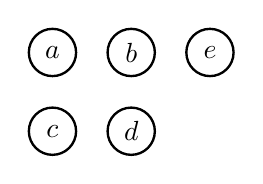
\begin{tikzpicture}
            \def \ax{0}   \def \ay{0}
            \def \bx{1}   \def \by{0}
            \def \cx{0}   \def \cy{-1}
            \def \dx{1}   \def \dy{-1}
            \def \ex{2}   \def \ey{0}

            \draw[line width=0.3mm] (\ax, \ay) circle (0.3) node[anchor=center]{$a$};
            \draw[line width=0.3mm] (\bx, \by) circle (0.3) node[anchor=center]{$b$};
            \draw[line width=0.3mm] (\cx, \cy) circle (0.3) node[anchor=center]{$c$};
            \draw[line width=0.3mm] (\dx, \dy) circle (0.3) node[anchor=center]{$d$};
            \draw[line width=0.3mm] (\ex, \ey) circle (0.3) node[anchor=center]{$e$};
            % Attacks
            \DrawSelfAttackRightSingleton{\ex}{\ey}
            \DrawAttackVertical{B}{\ax}{\ay}{\cx}{\cy}
            \DrawAttackHorizontal{R}{\ax}{\ay}{\bx}{\by}
            \DrawAttackHorizontal{L}{\dx}{\dy}{\cx}{\cy}
            \DrawAttackDiagonal{PLR}{\cx}{\cy}{\bx}{\by}
    
        \end{tikzpicture}
        \subcaption{\texttt{arg\_amount}=5 \texttt{p}=0.25}
        \label{af:ImplementationRandomBasedExampleAFsa}
    \end{minipage}
\begin{minipage}{.3\textwidth}
    \centering
    \begin{tikzpicture}
        % Singletons
        \def \ax{0}   \def \ay{0}
        \def \bx{1}   \def \by{0}
        \def \cx{1}   \def \cy{-1}
        \def \dx{2}   \def \dy{0}
        \def \ex{2}   \def \ey{-1}

        \draw[line width=0.3mm] (\ax, \ay) circle (0.3) node[anchor=center]{$a$};
        \draw[line width=0.3mm] (\bx, \by) circle (0.3) node[anchor=center]{$b$};
        \draw[line width=0.3mm] (\cx, \cy) circle (0.3) node[anchor=center]{$c$};
        \draw[line width=0.3mm] (\dx, \dy) circle (0.3) node[anchor=center]{$d$};
        \draw[line width=0.3mm] (\ex, \ey) circle (0.3) node[anchor=center]{$e$};

        % Attacks
        \DrawSelfAttackLeftSingleton{\ax}{\ay}
        \DrawSelfAttackRightSingleton{\dx}{\dy}
        \DrawSelfAttackRightSingleton{\ex}{\ey}
        \DrawAttackHorizontal{L}{\bx}{\by}{\ax}{\ay}
        \DrawAttackHorizontal{R}{\bx}{\by}{\dx}{\dy}
        \DrawAttackHorizontal{R}{\cx}{\cy}{\ex}{\ey}
        \DrawAttackVertical{D}{\dx}{\dy}{\ex}{\ey}
        \DrawAttackVertical{D}{\bx}{\by}{\cx}{\cy}
        \DrawAttackDiagonal{NLR}{\bx}{\by}{\ex}{\ey}
        \DrawAttackDiagonal{NRL}{\cx}{\cy}{\ax}{\ay}

        % Weird Attack
        \def \argSize{0.3}
        \draw[-{To[length=4, width=5]}, line width=0.3mm]
            (\ax + \argSize/2, \ay + \argSize - 0.05) .. controls
            (\bx-0.2 , \by + \argSize + 0.2) and
            (\bx+0.2 , \by + \argSize + 0.2) ..
            (\dx - \argSize/2, \dy + \argSize - 0.05);
    \end{tikzpicture}
    \subcaption{\texttt{arg\_amount}=5 \texttt{p}=0.5}
    \label{af:ImplementationRandomBasedExampleAFsb}
\end{minipage}%
\begin{minipage}{.3\textwidth}
    \centering
    \begin{tikzpicture}
        % Singletons
        \def \ax{0}   \def \ay{0}
        \def \bx{1}   \def \by{0}
        \def \cx{0}   \def \cy{-1}
        \def \dx{1}   \def \dy{-1}
        \def \ex{2}   \def \ey{0}

        \draw[line width=0.3mm] (\ax, \ay) circle (0.3) node[anchor=center]{$a$};
        \draw[line width=0.3mm] (\bx, \by) circle (0.3) node[anchor=center]{$b$};
        \draw[line width=0.3mm] (\cx, \cy) circle (0.3) node[anchor=center]{$c$};
        \draw[line width=0.3mm] (\dx, \dy) circle (0.3) node[anchor=center]{$d$};
        \draw[line width=0.3mm] (\ex, \ey) circle (0.3) node[anchor=center]{$e$};

        % Attacks
        \DrawSelfAttackLeftSingleton{\ax}{\ay}
        \DrawSelfAttackLeftSingleton{\cx}{\cy}
        \DrawSelfAttackRightSingleton{\ex}{\ey}
        \DrawAttackDiagonal{NB}{\ax}{\ay}{\dx}{\dy}
        \DrawAttackDiagonal{PB}{\bx}{\by}{\cx}{\cy}
        \DrawAttackHorizontal{L}{\bx}{\by}{\ax}{\ay}
        \DrawAttackHorizontal{R}{\cx}{\cy}{\dx}{\dy}
        \DrawAttackHorizontal{L}{\ex}{\ey}{\bx}{\by}
        \DrawAttackVertical{B}{\ax}{\ay}{\cx}{\cy}

        % Weird Attack
        \def \argSize{0.3}
        \draw[-{To[length=4, width=5]}, line width=0.3mm]
            (\ax + \argSize/2, \ay + \argSize - 0.05) .. controls
            (\bx-0.2 , \by + \argSize + 0.2) and
            (\bx+0.2 , \by + \argSize + 0.2) ..
            (\ex - \argSize/2, \ey + \argSize - 0.05);
    \end{tikzpicture}
    \subcaption{\texttt{arg\_amount}=5 \texttt{p}=0.75}
    \label{af:ImplementationRandomBasedExampleAFsc}
\end{minipage}
\caption{Example AF generated with random-based approach}
\label{fig:ImplementationRandomBasedExampleAFs}
\end{figure}
\vspace{0.3cm}



\paragraph{grid-based} Next we are going to discuss the grid-based approach. The arguments for the script are \texttt{<arg\_amount>}, being the amount of arguments the AF has and \texttt{<p>}, which is the probability that an attack between two arguments occurs. Different to the random-based approach, attacks can only happen between the direct neighbours of the grid (i.e.\ top, bottom, right, left). The grid is a $n \times n$ grid, with $n$ being equal to $\lfloor (\sqrt{\texttt{<arg\_amount>}}) \rfloor$. An example grid can be seen in \cref{fig:GridBasedApproach}.

\begin{figure}[h!]
    \centering
    \begin{tikzpicture}
        \def \rectSize{0.7cm}
        \def \rectSpace{0.5cm}

        \foreach \row in {0,1,2,3} {
            \foreach \col in {0,1,2,3} {
                \def \x{\rectSize * \col + \rectSpace * \col}
                \def \y{\rectSize * \row + \rectSpace * \row}
                \def \xArrowStart{\x+\rectSize/2}
                \def \xArrowEnd{\x+\rectSize/2+\rectSpace}
                \def \yArrowStart{\y+\rectSize/2}
                \def \yArrowEnd{\y+\rectSize/2+\rectSpace}

                % Rectangle
                \node[rectangle, draw, line width=0.3mm, minimum width=\rectSize, minimum height=\rectSize] at (\x, \y) {};

                \ifnum\col<3
                    % Arrow
                    \draw[dotted,<->, line width=0.3mm, >={To[length=4, width=5]}] (\xArrowStart,\y) -- (\xArrowEnd,\y);
                \fi

                \ifnum\row<3
                    % Arrow
                    \draw[dotted,<->, line width=0.3mm, >={To[length=4, width=5]}] (\x,\yArrowStart) -- (\x,\yArrowEnd);
                \fi
            }
        }
    \end{tikzpicture}
    \caption{Grid-Based Approach. $Amount=16$}
    \label{fig:GridBasedApproach}
\end{figure}

With the grid-based approach, we obtain a more structured AF. Structured in this context means, that the attacks between the arguments are restricted to locality. Due to this restriction, we reduce the amount of neighbours drastically in comparison to the random-based approach. Since we have less neighbours, we decrease the computation time and increase the chance to find a faithful AF.

\paragraph{level-based} The last approach we provide is the level-based approach. The arguments for this script are \texttt{<arg\_amount>}, \texttt{<level>} and \texttt{<p>}. Same as for the grid-based and random-based approach, \texttt{<arg\_amount>} defines how many arguments the computed AF has. The \texttt{<level>} argument restricts the height of the grid to the provided value and \texttt{<p>} is again the probability that an attack between to arguments occurs. The difference to the grid-based approach is the dimension of the grid. While the grid-based approach uses a $n \times n$ grid, in the level-based approach we use a $\texttt{<level>} \times n$ grid. In this context, $n$ is equal to $\lceil \texttt{<arg\_amount>}/2 \rceil$. An example grid is depicted in \cref{fig:LevelBasedApproach}.


\begin{figure}[h!]
    \centering
    \begin{tikzpicture}
        \def \rectSize{0.7cm}
        \def \rectSpace{0.5cm}

        \foreach \row in {0,1} {
            \foreach \col in {0,1,2,3,4,5,6,7} {
                \def \x{\rectSize * \col + \rectSpace * \col}
                \def \y{\rectSize * \row + \rectSpace * \row}
                \def \xArrowStart{\x+\rectSize/2}
                \def \xArrowEnd{\x+\rectSize/2+\rectSpace}
                \def \yArrowStart{\y+\rectSize/2}
                \def \yArrowEnd{\y+\rectSize/2+\rectSpace}

                % Rectangle
                \node[rectangle, draw, line width=0.3mm, minimum width=\rectSize, minimum height=\rectSize] at (\x, \y) {};

                \ifnum\col<7
                    % Arrow
                    \draw[dotted,<->, line width=0.3mm, >={To[length=4, width=5]}] (\xArrowStart,\y) -- (\xArrowEnd,\y);
                \fi

                \ifnum\row<1
                    % Arrow
                    \draw[dotted,<->, line width=0.3mm, >={To[length=4, width=5]}] (\x,\yArrowStart) -- (\x,\yArrowEnd);
                \fi
            }
        }
    \end{tikzpicture}
    \caption{Level-Based Approach. $Level=2$ and $Amount=16$}
    \label{fig:LevelBasedApproach}
\end{figure}





\section{BFS and DFS Approach}
\label{sec:ImplementationsBFSandDFSApproach}
\textit{TODO: BFS and DFS approach in current research + when BFS is better than DFS}







\section{Generating Semantics Sets}
\label{sec:ImplementationsGeneratingSemanticsSets}
\textit{TODO: Semantic sets generation algorithm}

\section{Faithful/Spurious Determination}
\label{sec:ImplementationsFaithfulSpuriousDetermination}
\textit{TODO: Determine faithful/spurious algorithm}

\section{Refuted Theories}
\label{sec:ImplementationsRefutedTheories}
\textit{TODO: State refuted theories like subsets of spurious also spurious.}




REUSE THIS SOMEWHERE:

We encoded the semantics rules into Boolean formula and used the SAT-Solver to evaluate them. To cover all possibilities of AFs, we generalized the formulas and used short notation to concatinate the variables. Let us have a look at a concrete example with an abstract clustered AF $\mathtt{\hat{G}=(\hat{A}, \hat{R})}$ defined in \cref{af:backgroundSATExample1}.



\begin{figure}[h]
    \centering
    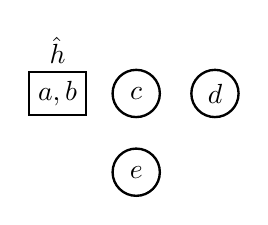
\begin{tikzpicture}
        % Singletons
        \def \cx{1}     \def \cy{0}
        \def \dx{2}     \def \dy{0}
        \def \ex{1}     \def \ey{-1}
        \def \hx{0}     \def \hy{0}

        \node[rectangle, draw, line width=0.3mm] at (\hx, \hy) {$a,b$};
        \node at (0, 0.55) {$\hat{h}$};
        \draw[line width=0.3mm] (\cx, \cy) circle (0.3) node[anchor=center]{$c$};
        \draw[line width=0.3mm] (\dx, \dy) circle (0.3) node[anchor=center]{$d$};
        \draw[line width=0.3mm] (\ex, \ey) circle (0.3) node[anchor=center]{$e$};

        % Attacks
        \DrawAttackHorizontal{R}{\hx+0.1}{\hy}{\cx}{\cy}
        \DrawSelfAttackRightSingleton{\cx}{\cy}
        \DrawAttackHorizontal{R}{\cx}{\cy}{\dx}{\dy}
        \DrawAttackVertical{D}{\cx}{\cy}{\ex}{\ey}
        \DrawAttackDiagonal{PB}{\dx}{\dy}{\ex}{\ey}
    \end{tikzpicture}
    \caption{Abstract AF $\mathtt{\hat{G}}$}
    \label{af:backgroundSATExample1}
\end{figure}


\paragraph{For-OR} To concatinate all the singletons of the AF $\hat{G}$, we can use the following notation:

$$
\bigvee_{a \in \hat{G}_{\!S\!I\!N\!G\!L\!E}} a = c \lor d \lor e
$$

\paragraph{For-AND} To concatinate all the singletons of the AF $\hat{G}$, we can use the following notation:

$$
\bigwedge_{a \in \hat{G}_{\!S\!I\!N\!G\!L\!E}} a = c \land d \land e
$$

\paragraph{For-Attacks} To iterate over the attacks $\hat{R}$ we can extract it from the AF as tuple and address the attacker $a$ and defender $b$:

$$
\bigwedge_{(a, b) \in \hat{R}, a\in \hat{G}_{\!S\!I\!N\!G\!L\!E}} \big( a \lor b \big) = (c \lor c) \land
(c \lor d) \land (c \lor e) \land (e \lor d) \land (d \lor e)
$$